\section[Conductance et résistance thermique]{Conductance et résistance thermique en régime permanent}
    \subsection{Analogie conduction thermique et électrique en régime permanent}

        On donne à la Table~\ref{tab:analogie_conduction_thermique_electrique} une comparaison entre les grandeurs et les lois apparaissant dans les phénomènes de conduction thermique et de conduction électricité.

        \begin{table}
            \centering
            \begin{tabular}{l|c|c}
                \toprule
                & thermique & électricité \\ \midrule
                Grandeur&&\\ transportée & énergie [\si[]{\joule}] & charge [\si[]{\coulomb}]\\ \midrule
                Vecteur&&\\ densité de courant & $\vec{j_\text{th}}$ [\si[]{\watt\per\metre\square}] & $\vec{j}$ [\si[]{\ampere\per\metre\square}]\\ \midrule
                Flux & $P_{\text{th}}=\iint_{S}\vec{j_\text{th}}\cdot\vec{dS}$ [\si[]{\watt}] & $i=\iint_{S}\vec{j}\cdot\vec{dS}$ [\si[]{\ampere}]\\ \midrule
                Équation locale&&\\de conservation&&\\ de l'énergie&&\\en régime permanent & $\div\vec{j_\text{th}}=0$ & $\div\vec{j}=0$\\ \midrule
                Loi de transport&&\\linéaire & $\vec{j_\text{th}}=-\lambda\vecgrad T$ & $\vec{j}=\sigma\vec{E}=-\sigma\vecgrad V$\\ &[Fourier]&[Ohm]\\\midrule
                Conductivité & $\lambda$ [\si[]{\watt\per\metre\per\kelvin}] & $\sigma$ [\si[]{\per\ohm\per\metre}]\\ \midrule
                Équation locale\\(en régime permanent) & $\Delta T=0$ & $\Delta V=0$\\ \bottomrule
            \end{tabular}    
            \caption{Analogie entre conduction thermique et électrique en régime permanent.}
            \label{tab:analogie_conduction_thermique_electrique}
        \end{table}

        Notons que l'on a le théorème d'unicité des solutions de $\Delta f=0$ pour une géométrie et des conditions aux limites données. On peut donc transposer des solutions d'un domaine à l'autre.

    \subsection{Résistance thermique conductive en une dimension}
        \subsubsection{Profil $T(x)$ en une dimension par conduction pure}

            On considère le système donnée à la Figure~\ref{fig:resistance_thermique_conductive_1d}.
            \begin{figure}
                \centering
                \tikzsetnextfilename{resistance_thermique_conductive_1d}
                \begin{tikzpicture}[scale=1]  
                    % \helpgrid{3}{3}
                    \draw[pattern=north west lines] (-3,1) rectangle++(6,0.25);
                    \draw[pattern=north west lines] (-3,-1.25) rectangle++(6,0.25);
                    \draw [dashed,->,-stealth] (-4,0)--++(8,0) node [right] {$x$};
                    \node at (-3.5,0.25) {$T_1$};
                    \node at (3.5,0.25) {$T_2$};
                    \node at (0,0.25) {$T(x)$};
                    \draw[latex-latex] (-3,-1.5)--++(6,0) node [below, midway] {$L$};

                    \draw[thick,line width=2pt] (-3,-1)--(-3,1);
                    \draw[thick,line width=2pt] (3,-1)--(3,1);

                \end{tikzpicture}
                \caption{Profil de température d'un système unidimensionnel pour établir l'expression de la résistance thermique.}    
                \label{fig:resistance_thermique_conductive_1d}
            \end{figure}

            On a $\Delta T=0=\dfrac{\rmd^{2}T}{\rmd x^{2}}$, donc $T(x)=\alpha+\beta x$. Avec les conditions aux limites, on a donc
            \begin{equation*}
                T(x)=T_1+\frac{T_2-T_1}{L}x.
            \end{equation*}
            Notons que l'on a $\vecgrad T=\dfrac{T_2-T_1}{L}\vec{u_x}=\vec{\mathrm{constance}}$.

        \subsubsection{Résistance thermique}

            Pour la conduction thermique, on a $R=\dfrac{U}{I}$. Ainsi, pour la conduction thermique, on devrait avoir une expression du type
            \begin{equation*}
                \frac{T_2-T_1}{R_{\text{th}}}=\dots
            \end{equation*}

            On a 
            \begin{align*}
                P_{\text{th}}
                &=\iint_{S}\vec{j_\text{th}}\cdot\vec{dS},\\
                &=
                -\lambda\frac{\rmd T}{\rmd x}S,\\
                &=
                \frac{\lambda(T_1-T_2)S}{L},\\
                &=\frac{\lambda S}{L}(T_1-T_2).
            \end{align*}

            Ainsi, on a 
            \begin{equation*}
                \boxed{
                    G_{\text{th}}=\frac{1}{R_{\text{th}}}=\frac{\lambda S}{L}.
                }
            \end{equation*}

            On a donc le schéma équivalent donné à la Figure~\ref{fig:schema_equivalent_resistance_conductance_thermique}.
            \begin{figure}
                \centering
                \tikzsetnextfilename{schema_equivalent_resistance_conductance_thermique}
                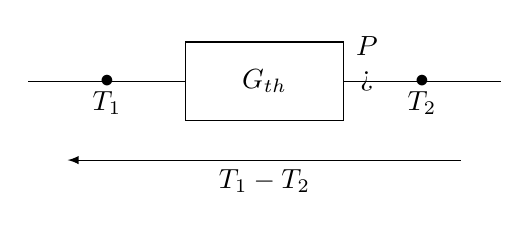
\begin{tikzpicture}[scale=1]  
                    % \helpgrid{3}{3}
                    \draw (-1,0) rectangle++(2,1);
                    \node at (0,0.5) {$G_{\text{th}}$};

                    \draw (-3,0.5)--(-1,0.5) node [midway] {$\bullet$};
                    \draw (1,0.5)--(3,0.5) node [midway] {$\bullet$};
                    \node at (-2,0.5) [below] {$T_1$};
                    \node at (2,0.5) [below] {$T_2$};
                    \draw [latex-] (-2.5,-0.5)--++(5,0) node [below, midway] {$T_1-T_2$};
                    \node at (1.3,0.5) {>};
                    \node at (1.3,0.5) [above,shift={(0,0.2)}] {$P$};
                \end{tikzpicture}
                \caption{Schéma équivalent pour la résistance/conductance thermique.}    
                \label{fig:schema_equivalent_resistance_conductance_thermique}
            \end{figure}

            C'est la même chose pour une géométrie cylindrique ou sphérique.

    \subsection{Résistance thermique conducto-convective}

        On reprend le système décrit à la Figure~\ref{fig:transfert_conducto_convectif_fluide_brasse}. On a 
        \begin{equation*}
            P_{\text{th}}^{\text{cc}}=\varphi_{\text{cc}}S=h(T_s-T_f)=hS(T_s-T_f),    
        \end{equation*}
        soit
        \begin{equation*}
            \boxed{
                G_{\text{cc}}=\frac{1}{R_{\text{cc}}}=hS.
            }
        \end{equation*}

    \subsection{Association en série : résistance \og multicouche\fg}

        On prend l'exemple d'um mur comprenant une couche de plâtre, d'isolant puis de pierre, voir la Figure~\ref{fig:exemple_association_serie_resistance_thermique}.

        \begin{figure}
            \centering
            \tikzsetnextfilename{exemple_association_serie_resistance_thermique}
            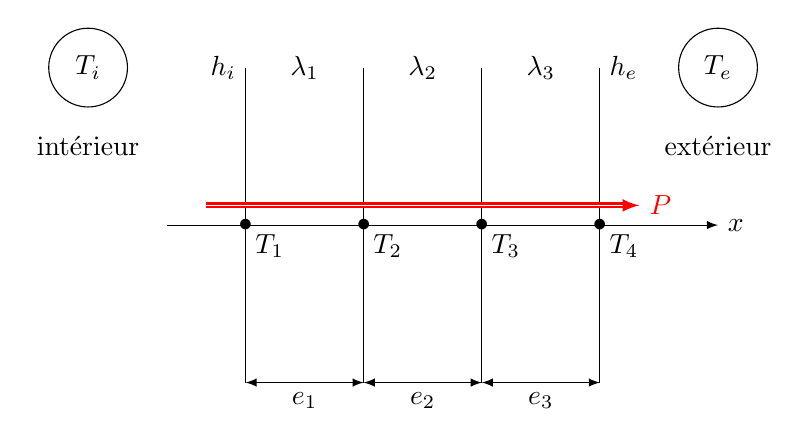
\begin{tikzpicture}[scale=1]  
                % \helpgrid{3}{3}
                \draw[-latex] (-3,0)--(4,0) node [right] {$x$};
                \node at (-2,0) {$\bullet$};
                \node at (-0.5,0) {$\bullet$};
                \node at (1,0) {$\bullet$};
                \node at (2.5,0) {$\bullet$};

                \node at (-2,0) [below right] {$T_1$};
                \node at (-0.5,0) [below right] {$T_2$};
                \node at (1,0) [below right] {$T_3$};
                \node at (2.5,0) [below right] {$T_4$};

                \node at (-4,1) {intérieur};
                \node at (4,1) {extérieur};
                \draw [smooth] (-4,2) circle (0.5) node {$T_i$};
                \draw [smooth] (4,2) circle (0.5) node {$T_e$};

                \draw (-2,-2)--++(0,4) node [left] {$h_i$};
                \draw (-0.5,-2)--++(0,4);
                \draw (1,-2)--++(0,4);
                \draw (2.5,-2)--++(0,4) node [right] {$h_e$};

                \draw [double, -latex, thick, red, text=red] (-2.5,0.25)--++(5.5,0) node [right] {$P$};

                \draw [latex-latex] (-2,-2)--(-0.5,-2) node [below, midway] {$e_1$};
                \draw [latex-latex] (-0.5,-2)--(1,-2) node [below, midway] {$e_2$};
                \draw [latex-latex] (1,-2)--(2.5,-2) node [below, midway] {$e_3$};

                \node at (-1.25,2) {$\lambda_1$};
                \node at (0.25,2) {$\lambda_2$};
                \node at (1.75,2) {$\lambda_3$};
            \end{tikzpicture}
            \caption{Exemple d'association de résistances en série : cas d'un mur.}    
            \label{fig:exemple_association_serie_resistance_thermique}
        \end{figure}

        La même puissance $P$ traverse toutes les couches : \textbf{elles sont montées en série}. On a alors
        \begin{align*}
            P
            &=h_iS(T_i-T_1)=\frac{\lambda_1 S}{e_1}(T_1-T_2),\\
            &=\frac{\lambda_2 S}{e_2}(T_2-T_3)=\frac{\lambda_3 S}{e_3}(T_4-T_3)=h_e S(T_4-T_e).
        \end{align*}

        Ainsi,
        \begin{align*}
            T_i-T_e
            &=
            (T_i-T_1)+(T_1-T_2)+(T_2-T_3)+(T_3-T_4)+(T_4-T_e),\\
            &=\left[
                \frac{1}{h_i S}+\frac{e_1}{\lambda_1 S}+\frac{e_2}{\lambda_2 S}+\frac{e_3}{\lambda_3 S}+\frac{1}{h_e S}
            \right]P.
        \end{align*}
        Ainsi,
        \begin{equation*}
            T_i-T_e=R_{\text{th}}^{\text{eq}}P,
        \end{equation*}
        avec la résistance équivalente donnée par
        \begin{equation*}
            \boxed{
                R_{\text{th}}^{\text{eq}}=\sum_{i}R_{\text{th},i}.
            }
        \end{equation*}

        Le schéma équivalent est donné à la Figure~\ref{fig:schema_equivalent_association_serie_resistance_thermique}.

        \begin{figure}
            \centering
            \tikzsetnextfilename{schema_equivalent_association_serie_resistance_thermique}
            \begin{tikzpicture}[scale=0.9]  
                % \helpgrid{3}{3}
                
                \coordinate (Ti) at (-0.5,0);
                \coordinate (T1) at (2,0);
                \coordinate (T2) at (4.5,0);
                \coordinate (T3) at (7,0);
                \coordinate (T4) at (9.5,0);
                \coordinate (Te) at (12,0);

                
                \node at (12.5,0) {>};
                \node at (12.5,0) [above,shift={(0,0.2)}] {$P$};
                \node at (Ti) {$\bullet$};
                \node at (T1) {$\bullet$};
                \node at (T2) {$\bullet$};
                \node at (T3) {$\bullet$};
                \node at (T4) {$\bullet$};
                \node at (Te) {$\bullet$};
                \node at (Ti) [above] {$T_i$};
                \node at (T1) [above] {$T_1$};
                \node at (T2) [above] {$T_2$};
                \node at (T3) [above] {$T_3$};
                \node at (T4) [above] {$T_4$};
                \node at (Te) [above] {$T_e$};

                \draw (0,-0.5) rectangle++(1.5,1);
                \node at (0.75,0) {$\dfrac{1}{h_iS}$};
                \draw (2.5,-0.5) rectangle++(1.5,1);
                \node at (3.25,0) {$\dfrac{e_1}{\lambda_1S}$};
                \draw (5,-0.5) rectangle++(1.5,1);
                \node at (5.75,0) {$\dfrac{e_2}{\lambda_2S}$};
                \draw (7.5,-0.5) rectangle++(1.5,1);
                \node at (8.25,0) {$\dfrac{e_3}{\lambda_3S}$};
                \draw (10,-0.5) rectangle++(1.5,1);
                \node at (10.75,0) {$\dfrac{1}{h_eS}$};
                
                \draw (-1,0)--(0,0);
                \draw (1.5,0)--(2.5,0);
                \draw (4,0)--(5,0);
                \draw (6.5,0)--(7.5,0);
                \draw (9,0)--(10,0);
                \draw (11.5,0)--(13,0);


            \end{tikzpicture}
            \caption{Schéma équivalent pour l'association en série de résistances thermiques.}    
            \label{fig:schema_equivalent_association_serie_resistance_thermique}
        \end{figure}

        Ici, l'isolant est prédominant : on a $R_{\text{th}}^{\text{eq}}\approx R_{\text{th}}^{\text{iso}}=\dfrac{e_2}{\lambda_2S}$.

    \subsection{Association en parallèle}

        On prend l'exemple d'un mur percé d'une fenêtre, que l'on modélise à la Figure~\ref{fig:exemple_association_parallele_resistance_thermique}.

        \begin{figure}
            \centering
            \tikzsetnextfilename{exemple_association_parallele_resistance_thermique}
            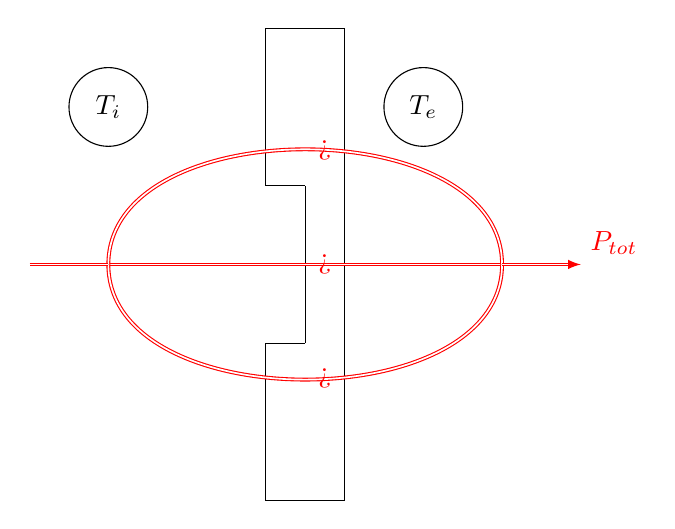
\begin{tikzpicture}[scale=1]  
                % \helpgrid{3}{3}
                
                \draw (0,3)--(1,3);
                \draw (1,3)--(1,-3);
                \draw (0,-3)--(1,-3);
                \draw (0,3)--(0,1);
                \draw(0,-3)--(0,-1);
                \draw (0,1)--(0.5,1);
                \draw (0,-1)--(0.5,-1);
                \draw (0.5,-1)--(0.5,1);

                \draw (-2,2) circle (0.5) node {$T_i$};
                \draw (2,2) circle (0.5) node {$T_e$};

                \draw[double, red] (-2,0) to (3,0);
                \draw[double, red, bend left=90] (-2,0) to (3,0);
                \draw[double, red, bend right=90] (-2,0) to (3,0);
                \draw[double, red] (-3,0) to (-2,0);
                \draw[double, red,-latex] (3,0) to (4,0) node [above right] {$P_{\text{tot}}$};

                \node [text=red] at (0.75,0) {>};
                \node [text=red] at (0.75,1.45) {>};
                \node [text=red] at (0.75,-1.45) {>};
            \end{tikzpicture}
            \caption{Exemple d'association en parallèle de résistances thermiques.}    
            \label{fig:exemple_association_parallele_resistance_thermique}
        \end{figure}

        L'équivalent de la loi des n\oe uds donne
        \begin{equation*}
            \boxed{
                P_{\text{tot}}=P_{\text{mur}}+P_{\text{fenêtre}}.
            }
        \end{equation*}

        Le schéma équivalent est donné à la Figure~\ref{fig:schema_equivalent_association_parallele_resistance_thermique}.
        \begin{figure}
            \centering
            \tikzsetnextfilename{schema_equivalent_association_parallele_resistance_thermique}
            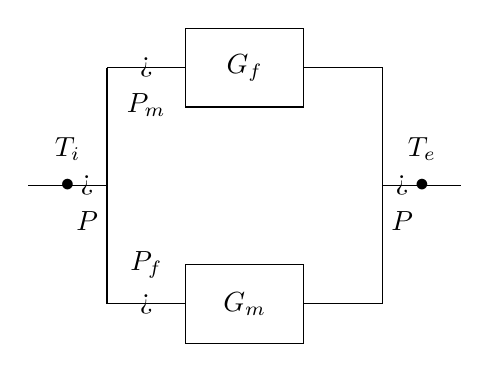
\begin{tikzpicture}[scale=1]  
                % \helpgrid{3}{3}

                \draw (0,1) rectangle++(1.5,1);
                \node at (0.75,1.5) {$G_f$};
                \draw (0,-2) rectangle++(1.5,1);
                \node at (0.75,-1.5) {$G_m$};

                \draw (-2,0)--(-1,0);
                \draw (-1,0)--(-1,1.5);
                \draw (-1,0)--(-1,-1.5);
                \draw (-1,1.5)--(0,1.5);
                \draw (-1,-1.5)--(0,-1.5);
                \draw (1.5,1.5)--(2.5,1.5);
                \draw (1.5,-1.5)--(2.5,-1.5);
                \draw (2.5,1.5)--(2.5,0);
                \draw (2.5,-1.5)--(2.5,0);
                \draw (2.5,0)--(3.5,0);

                \node at (-1.5,0) {$\bullet$};
                \node at (3,0) {$\bullet$};
                \node at (-1.5,0) [above,shift={(0,0.2)}] {$T_i$};
                \node at (3,0) [above,shift={(0,0.2)}] {$T_e$};
                \node at (-1.25,0) {>};
                \node at (-0.5,-1.5) {>};
                \node at (-0.5,1.5) {>};
                \node at (2.75,0) {>};
                \node at (-1.25,0) [below,shift={(0,-0.2)}] {$P$};
                \node at (-0.5,-1.5) [above,shift={(0,0.2)}] {$P_f$};
                \node at (-0.5,1.5) [below,shift={(0,-0.2)}] {$P_m$};
                \node at (2.75,0) [below,shift={(0,-0.2)}] {$P$};
            
            \end{tikzpicture}
            \caption{Schéma équivalent pour l'exemple d'association en parallèle de résistances thermiques.}    
            \label{fig:schema_equivalent_association_parallele_resistance_thermique}
        \end{figure}

        Ainsi,
        \begin{equation*}
            P_{\text{tot}}=G_f\times(T_i-T_e)+G_m\times(T_i-T_e)=G_{\text{eq}}\times(T_i-T_e),
        \end{equation*}
        avec
        \begin{equation*}
            \boxed{
                G_{\text{eq}}=\sum_{i}G_i,\qquad \frac{1}{R_{\text{th}}^{\text{eq}}}=\sum_{i}\frac{1}{R_{\text{th,i}}}.
            }
        \end{equation*}

        Il y a un \og court-circuit thermique\fg. Notamment, s'il y a un pont thermique, alors $G_{\text{pont}}\gg G_i$ et ainsi $G_{\text{eq}}\approx G_{\text{pont}}$.

    \subsection{ARQS en thermique}

        \subsubsection{Exemple : circuit thermique dans l'ARQS}

            On considère une chambre dont un côté donne sur l'extérieur (et les trois autres vers l'intérieur), voir la Figure~\ref{fig:ARSQ_thermique_exemple}.
            \begin{figure}
                \centering
                \tikzsetnextfilename{ARSQ_thermique_exemple}
                \begin{tikzpicture}[scale=1]  
                    % \helpgrid{3}{3}
    
                    \draw (0,0) rectangle++(2,2);
                    \node at (1,1) {$T(t)$};
                    \node at (-1,1) {$T_i$};
                    \node at (1,3) {$T_i$};
                    \node at (1,-1) {$T_i$};
                    \node at (3,1) {$T_e$};
                
                \end{tikzpicture}
                \caption{Exemple de de l'ARQS en thermique.}    
                \label{fig:ARSQ_thermique_exemple}
            \end{figure}

            On suppose que l'on a les paramètres suivants : pour le côté extérieur, on a la conductance $G_e$, pour le côté intérieur on a la conductance $G_i$, pour la pièce il y a un chauffage $P_{\text{ch}}>0$ en \si{\watt}, et la capacité thermique de la chambre est $C$ en \si{\joule\per\kelvin}. Alors on a

            \begin{equation*}
                \frac{\rmd U}{\rmd t}=C\frac{\rmd T}{\rmd t}=P_{\text{ch}}-G_e(T(t)-T_e)-G_i(T(t)-T_i).
            \end{equation*}

            Ainsi,
            \begin{equation*}
                \frac{\rmd T}{\rmd t}+\frac{G_e+G_i}{C}T=\frac{P_{\text{ch}}+G_e T_e+G_i T_i}{C},
            \end{equation*}
            ce qui donne le schéma équivalent donné à la Figure~\ref{fig:ARQS_schema_equivalent}.

            \begin{figure}
                \centering
                \tikzsetnextfilename{ARQS_schema_equivalent}
                \begin{circuitikz} 
                    \draw (0,0) -- (0,0) node[ground]{}; 
                    \draw (0,0) to[C,l=$C$] (0,3);

                    \draw (2,0) -- (2,0) node[ground]{}; 
                    \draw (2,0) to[european current source,l=$P_{\text{ch}}$] (2,3);

                    \draw (4,0) -- (4,0) node[ground]{}; 
                    \draw (4,0) to[european voltage source, l=$T_e$] (4,1) to[generic,l=$G_e$] (4,3);

                    \draw (6,0) -- (6,0) node[ground]{}; 
                    \draw (6,0) to[european voltage source, l=$T_i$] (6,1) to[generic,l=$G_i$] (6,3);
                    \draw (0,3)--(6,3);
                    \node at (4,3) {$\bullet$};
                    \node at (4,3) [above] {$T(t)$};

                    \node at (0,2.5) {$\bullet$};
                    \node at (0,2.5) [right] {$T(t)$};
                    \draw[-latex] (-1,1)--(-1,2.5) node [left, midway] {$T(t)$};
                    
                    \end{circuitikz}
                \caption{Schéma équivalent dans l'ARQS thermique}    
                \label{fig:ARQS_schema_equivalent}
            \end{figure}

            On pose 
            \begin{equation*}
                \boxed{
                    \frac{1}{\tau}=\frac{G_{\text{eq}}}{C},
                }
            \end{equation*}
            et on obtient
            \begin{equation*}
                T(t)=A\rme^{-t/\tau}+\frac{P_{\text{ch}}}{G_e+G_i}+\frac{G_e T_e+G_i T_i}{G_e+G_i}.
            \end{equation*}
            On résout ensuite avec d'éventuelles conditions initiales.

        \subsubsection{Qu'est-ce que l'ARQS ?}
            Ce qu'on a écrit suppose la validité du concept de résistance thermique. Dans chaque couche, on doit donc avoir un profil $T(x)$ environ affine. Cela suppose une diffusion thermique quasi instantanée, c'est-à-dire 
            \begin{equation*}
                \tau_{\text{diff}}\sim\frac{e^{2}}{D_{\text{th}}}\ll t,
            \end{equation*}
            i.e.~$F_0(t)\gg1$, c'est-à-dire
            \begin{equation*}
                \boxed{
                    t\gg\frac{e^{2}}{\frac{\lambda}{\mu c}},
                }
            \end{equation*}
            dans chaque couche d'épaisseur $e$.